\documentclass[conference,a4paper]{IEEEtran}
\IEEEoverridecommandlockouts

\usepackage{amsmath,amssymb,amsfonts}
\usepackage{algorithmic}
\usepackage{graphicx}
\usepackage{textcomp}
\usepackage{xcolor}
\usepackage{booktabs}
\usepackage{url}
\usepackage{cite}
\usepackage{tikz}
\usetikzlibrary{arrows.meta, positioning, calc, shapes.geometric, fit, backgrounds, decorations.pathreplacing}

% Shared notation macros
\newcommand{\SCU}{\text{SCU}}
\newcommand{\Cost}{\text{Cost}}
\newcommand{\CPM}{C_{\text{PM}}}
\newcommand{\CFAIL}{C_{\text{FAIL}}}
\newcommand{\CWASTE}{C_{\text{WASTE}}}
\newcommand{\MPIW}{\text{MPIW}}
\newcommand{\RUL}{\text{RUL}}
\newcommand{\Deltacost}{\Delta_{\text{cost}}}
\newcommand{\Deltaerror}{\Delta_{\text{error}}}
\newcommand{\Deltafail}{\Delta_{\text{fail}}}
\newcommand{\Dwidth}{D_{\text{width}}}
\newcommand{\Dscore}{D_{\text{score}}}
\newcommand{\WorstErr}{\text{WorstErr}}
\newcommand{\WorstRegime}{\text{WorstRegime}}
\newcommand{\WorstStage}{\text{WorstStage}}
\newcommand{\RULtrue}{y}
\newcommand{\RULpred}{p}
\newcommand{\LowerBound}{L}
\newcommand{\UpperBound}{U}
\newcommand{\qglobal}{q_{\text{global}}}
\newcommand{\qregime}{q_k}
\newcommand{\qfinal}{q^*}
\newcommand{\sigmap}{\sigma(p)}
\newcommand{\zp}{z(p)}
\newcommand{\ap}{a(p)}
\newcommand{\bp}{b(p)}

\begin{document}

\title{IntelliTwin: Decision-Aware, Condition-Adaptive Conformal Prediction for Industrial Turbofan Predictive Maintenance}

\author{
\IEEEauthorblockN{Shiksha Pandey\IEEEauthorrefmark{1}, Mayank Singh\IEEEauthorrefmark{2}}
\IEEEauthorblockA{\IEEEauthorrefmark{1}Department of Information Technology, Ajay Kumar Garg Engineering College (AKGEC), Ghaziabad, India\\
\IEEEauthorrefmark{2}Department of Information Technology, Ajay Kumar Garg Engineering College (AKGEC), Ghaziabad, India}
}

\maketitle

\begin{abstract}
In industrial predictive maintenance of gas turbine engines, unexpected mechanical failure incurs severe airworthiness risks and catastrophic economic penalties ($5\times$ to $10\times$ scheduled overhaul), while premature overhaul discards valuable residual component life. Conventional Remaining Useful Life (RUL) prognostic architectures rely on deterministic point estimators that optimize symmetric cycle error metrics without quantifying prediction variance or aligning with downstream maintenance costs. Standard inductive conformal prediction provides marginal coverage guarantees but conceals severe conditional undercoverage across accelerating degradation stages and varying operating regimes. In this work, we present \textbf{IntelliTwin}, an uncertainty-aware prognostic framework integrating Gradient Boosted Regressors (GBR) and Long Short-Term Memory (LSTM) networks with hierarchical, decision-aware conformal calibration. IntelliTwin enforces strictly disjoint engine-level partitioning, causal temporal windowing ($w=30$, stride 1), exact rational engine weighting ($m/(m+1)$ mass), and an asymmetric nonconformity score parameterized by scale dilation ($\gamma=2$) and directional asymmetry ($\beta=-\ln 2$). We evaluate the framework under a frozen confirmatory protocol on 122 held-out test engines from NASA C-MAPSS sub-corpora FD001, FD002, and FD004 across 10,000 lifetime-stratified cluster-bootstrap draws with Bonferroni-controlled 98.75\% decision intervals. In confirmatory testing, the proposed method achieved substantial maintenance cost reductions ($+7.50$ to $+11.32$ Simulated Cost Units per engine on FD002) with zero fleet failures. However, under preregistered Intersection-Union Testing criteria, RQ1--RQ4 were formally classified as UNSUPPORTED because late-stage degradation coverage error breached the 0.05 ceiling ($E_{\text{stage}} \approx 0.13$, empirical coverage $\sim 77\%$). Through post-confirmatory factorial ablation across 240 cells, we isolate that scale dilation ($\gamma$) reduces cost by an unweighted mean of $-10.48$ SCU and directional asymmetry ($\beta$) reduces cost by $-1.21$ SCU, whereas regime routing provides null effects on single-condition fleets and small cost penalties ($+0.56$ SCU) on multi-condition fleets due to partition sample dispersion. Finally, we provide an open, fully reproducible historical validation-telemetry replay prototype.
\end{abstract}

\begin{IEEEkeywords}
Predictive Maintenance, Remaining Useful Life, Digital Twin, Conformal Prediction, Uncertainty Quantification, Condition-Adaptive Calibration, Turbofan Engines, C-MAPSS.
\end{IEEEkeywords}

\section{Introduction}

Prognostics and Health Management (PHM) for high-value rotating machinery has emerged as a cornerstone of operational safety and economic sustainability across commercial aviation, energy generation, and advanced manufacturing \cite{saxena2008damage, diana2025ai}. In commercial aircraft gas turbine turbofans, unscheduled engine removals and catastrophic in-flight failures impose disproportionate costs---frequently exceeding scheduled overhaul expenses by five- to ten-fold---while posing critical flight safety risks \cite{shehadeh2024evaluating, hosseinzadeh2023predictive}. Conversely, legacy time-based preventative maintenance discards substantial remaining operational lifespan, severely inflating life-cycle overhaul expenditure \cite{bello2024ai, brighenti2024forecasting}.

Modern data-driven prognostic paradigms utilize multi-sensor telemetry to predict an asset's Remaining Useful Life (RUL) \cite{wu2026research}. Deep learning models, including Long Short-Term Memory (LSTM) networks and gradient-boosted regression ensembles, have achieved impressive cycle-level error reductions on standardized run-to-failure benchmarks such as NASA C-MAPSS \cite{saxena2008damage, diao2026turbofan}. However, standard point-regression models suffer from three structural shortcomings when deployed into operational maintenance decision pipelines:
\begin{enumerate}
    \item \textbf{Unquantified Point Variance}: A single deterministic cycle estimate provides no measure of epistemic or aleatoric uncertainty, preventing operators from distinguishing high-confidence prognostic estimates from high-risk extrapolations \cite{chen2022data, walia2026uncertainty}.
    \item \textbf{Conditional Reliability Breakdown}: Inductive split conformal prediction has emerged as an attractive, distribution-free methodology to construct finite-sample prediction intervals $[L, U]$ with marginal coverage guarantees $\mathbb{P}(y \in [L, U]) \ge 1 - \alpha$ \cite{javanmardi2023conformal, diao2026turbofan}. Nevertheless, marginal coverage guarantees do not ensure conditional coverage across varying operating regimes or accelerating wear stages \cite{yang2026empirical, yan2026audit}. In turbofan engines subject to dynamic throttle and atmospheric variations, standard conformal calibrators frequently undercover in late degradation phases where accurate risk bounds are most critical.
    \item \textbf{Decoupling of Uncertainty from Economic Consequences}: Standard prognostic objectives minimize symmetric errors (RMSE, MAE). In operational aviation maintenance, overestimating RUL leads to uncontained mechanical breakdown, whereas underestimating RUL causes only premature overhaul waste \cite{zhu2025predictive, robinson2026riskaware}. Symmetric prediction intervals fail to reflect this severe operational loss asymmetry.
\end{enumerate}

To bridge this operational and theoretical gap, we introduce \textbf{IntelliTwin}, an AI-driven framework that unifies deep sequence modeling, hierarchical conformal calibration, and asymmetric sequential maintenance simulation within an interactive Digital Twin replay architecture. 

The principal contributions of this research are:
\begin{itemize}
    \item \textbf{Decision-Aware Asymmetric Nonconformity}: We formulate an RUL-specific nonconformity scoring metric incorporating state-dependent horizon dilation ($\gamma=2$) and directional asymmetry ($\beta=-\ln 2$), skewing prediction interval bounds to penalize dangerous over-estimation while bounding premature intervention.
    \item \textbf{Hierarchical Engine-Weighted Calibration}: We implement an exact rational engine-weighting calibration scheme with mass $\frac{m}{m+1}$ on finite calibration scores and $\frac{1}{m+1}$ at $+\infty$, enforcing exchangeability at the physical engine level rather than pooling autocorrelated cycles.
    \item \textbf{Preregistered Confirmatory Evaluation}: We execute a strictly pre-frozen evaluation protocol across 122 held-out test engines from NASA C-MAPSS FD001, FD002, and FD004. In confirmatory testing, the proposed method achieved substantial maintenance cost reductions ($+7.50$ to $+11.32$ SCU/engine) with zero fleet failures. Under preregistered Intersection-Union Testing (IUT), RQ1--RQ4 were formally classified as UNSUPPORTED because late-stage coverage error breached the 0.05 ceiling ($E_{\text{stage}} \approx 0.13$).
    \item \textbf{Post-Confirmatory Factorial Ablation \& Stress Analysis}: Through an independent reference-audited $2 \times 2 \times 2$ factorial ablation across 240 cells and 1,620 stress evaluations, we demonstrate that scale dilation ($\gamma$) and directional asymmetry ($\beta$) drive cost reductions ($-10.48$ and $-1.21$ SCU, respectively), whereas regime routing introduces variance penalties on multi-condition fleets.
    \item \textbf{Digital Twin Telemetry Replay Prototype}: We implement an open-source, causal-windowed ($w=30$, zero lookahead) telemetry replay prototype with verified numerical parity ($\text{atol} \le 10^{-4}$) against validation predictions.
\end{itemize}

\section{Related Work}

\subsection{Prognostics and RUL Estimation}
Data-driven RUL estimation has evolved from classical statistical hazard modeling (Weibull, degradation filters) to complex neural architectures \cite{saxena2008damage}. Modern benchmarks heavily leverage the NASA Commercial Modular Aero-Propulsion System Simulation (C-MAPSS) dataset, which models 90,000-lb thrust turbofan degradation under mixed sea-level and high-altitude flight envelopes \cite{saxena2008damage, diao2026turbofan}. While recurrent and convolutional architectures achieve low RMSE, raw point predictions provide insufficient assurance for mission-critical dispatch \cite{wu2026research, belay2026digital}.

\subsection{Uncertainty Quantification in PHM}
Bayesian neural networks, Monte Carlo dropout, and deep ensemble methods have been investigated to estimate RUL variance \cite{chen2022data, xu2026novel}. However, Bayesian methods require strong prior assumptions, and ensemble variances often lack empirical coverage guarantees under distribution shift. Conformal prediction addresses this limitation by producing distribution-free, finite-sample prediction intervals \cite{javanmardi2023conformal}. Javanmardi and H\"ullermeier \cite{javanmardi2023conformal} demonstrated split conformal prediction on C-MAPSS FD001. Diao et al. \cite{diao2026turbofan} coupled LSTM quantile regression with conformal calibration. However, prior studies evaluated conformal intervals using standard symmetric coverage (PICP) and width (MPIW) metrics, overlooking the economic consequences of bound failures in sequential decision-making.

\subsection{Digital Twins and Decision-Directed Conformal Inference}
Digital Twins combine sensor telemetry, virtual models, and real-time state synchronization to track physical degradation \cite{huang2021survey, hasan2025new, pathri2025smart}. Recent theoretical developments by Cortes-Gomez et al. \cite{cortesgomez2025utility} formalized utility-directed conformal prediction for static decision problems, while Lee et al. \cite{lee2023hierarchical} established distribution-free inference for hierarchical data. Robinson \cite{robinson2026riskaware} introduced risk-aware conformal quantile regression for aircraft engines. IntelliTwin builds upon these foundations by unifying hierarchical engine weighting, state-dependent nonconformity scaling, and sequential discrete maintenance simulation into a single reproducible framework.

\section{Problem Formulation and Research Objectives}

\subsection{Degradation Process and Temporal Windowing}
Let an industrial turbofan engine $i \in \{1, \dots, N\}$ operate across discrete operational cycles $t \in \{1, \dots, T_i\}$, where $T_i$ denotes the terminal cycle of functional failure. At each cycle $t$, a vector of operational settings and sensor measurements $\mathbf{s}_{i,t} \in \mathbb{R}^{D}$ is observed. Observations are buffered into causal sliding windows of fixed length $w=30$ with unit stride:
\begin{equation}
\mathbf{X}_{i,t} = [\mathbf{s}_{i,t-w+1}, \dots, \mathbf{s}_{i,t}]^T \in \mathbb{R}^{w \times D}, \quad \forall t \ge w.
\end{equation}
Cycles $t < w$ constitute a non-predictive warm-up horizon. The true remaining useful life at observation endpoint $t$ is $y_{i,t} = T_i - t$. During model training, target values are clipped according to standard industry practice: $y_{\text{train}} = \min(y_{i,t}, R_{\text{max}})$, with $R_{\text{max}} = 125$ cycles. During evaluation and maintenance simulation, the true uncapped remaining life $y_{i,t}$ is evaluated.

\subsection{Sequential Maintenance Simulator Contract}
We model asset maintenance as a discrete-time stopping problem over cycles $t \in [w, T_i - 1]$. At each cycle, the decision agent observes telemetry history $\mathbf{X}_{i,t}$, computes calibrated lower bound $L(t)$, and executes an action $a_t \in \{\text{CONTINUE}, \text{MAINTAIN\_NOW}\}$ according to the policy:
\begin{equation}
a_t = \begin{cases} 
\text{MAINTAIN\_NOW} & \text{if } L(t) \le 1.0 \text{ cycle}, \\ 
\text{CONTINUE} & \text{otherwise}. 
\end{cases}
\end{equation}
If proactive maintenance is triggered at cycle $t_{\text{action}} < T_i$, the engine is removed from service, incurring preventive replacement cost $\CPM$ plus wasted life penalty proportional to discarded cycles:
\begin{equation}
\Cost(i) = \CPM + \CWASTE \cdot (T_i - t_{\text{action}}).
\end{equation}
If no maintenance action is triggered and the engine reaches terminal cycle $T_i$, catastrophic in-service failure occurs, incurring heavy penalty $\Cost(i) = \CFAIL$. Under the primary reference economic scenario, costs are set to $\CPM = 1.0$, $\CFAIL = 5.0$, and $\CWASTE = 0.20$ Simulated Cost Units (SCU) per engine.

\subsection{Formal Research Questions}
We establish four preregistered research questions:
\begin{itemize}
    \item \textbf{RQ1 (Sequential Utility)}: Can decision-aware conformal calibration improve sequential maintenance utility ($\Deltacost > 0.20$ SCU) while preserving prediction-interval coverage ($E < 0.05$)?
    \item \textbf{RQ2 (Conditional Reliability)}: Can the proposed method improve worst-group conditional coverage ($\Deltaerror > 0.01$) without excessive interval widening ($\Dwidth < 1.0$ cycle)?
    \item \textbf{RQ3 (Attribution)}: Are maintenance benefits attributable to decision-aware calibration rather than simple over-conservatism or premature intervention?
    \item \textbf{RQ4 (Robustness)}: Does the method retain calibration and utility benefits across operating conditions, base models, and datasets?
\end{itemize}

\section{Proposed IntelliTwin Framework}

The architecture of IntelliTwin comprises five decoupled stages:
\begin{enumerate}
    \item \textbf{Engine-Disjoint Data Pipeline}: Strict partitioning by physical engine ID prevents cross-trajectory leakage.
    \item \textbf{Prognostic Base Models}: Dual architectures (tree-based GBR and recurrent LSTM) trained on clipped RUL targets.
    \item \textbf{Asymmetric Conformal Scoring Engine}: Nonconformity scores parameterized by life-horizon dilation and risk asymmetry.
    \item \textbf{Hierarchical Engine Calibration}: Exact rational probability weighting ensuring valid distribution-free coverage.
    \item \textbf{Sequential Maintenance Simulator}: Discrete cycle evaluation translating lower bounds into realized maintenance costs.
\end{enumerate}

\section{Mathematical Methodology}

\subsection{Asymmetric Decision-Aware Nonconformity Scoring}
Let $p = \max(0, \hat{y})$ denote the non-negative evaluated point prediction in cycles, and let $y$ denote the true Remaining Useful Life. The asymmetric nonconformity score scales deviations according to state-dependent shape factors:
\begin{align}
\sigmap &= \left(1 + \frac{p}{125}\right)^\gamma, \quad \zp = \exp\left(-\frac{p}{20}\right), \\
\ap &= \sigmap \exp(\beta \zp), \quad \bp = \sigmap \exp(-\beta \zp),
\end{align}
where $\gamma \in \{0, 1, 2\}$ controls variance dilation with life horizon, and $\beta \in \{-\ln 2, 0, +\ln 2\}$ governs directional risk asymmetry. The nonconformity score is defined as:
\begin{equation}
\text{score}(p, y) = \max\left(\frac{p - y}{\ap}, \frac{y - p}{\bp}, 0\right).
\end{equation}
Inverting this score with respect to a calibrated quantile threshold $q^*$ produces valid prediction interval bounds:
\begin{equation}
\LowerBound = \max(0, p - q^* \cdot \ap), \quad \UpperBound = p + q^* \cdot \bp.
\end{equation}
Validation grid search across candidate pairs uniquely selected $\gamma = 2, \beta = -\ln 2 \approx -0.693147$.

\subsection{Hierarchical Engine-Weighted Calibration}
In final conformal calibration on $m$ reserved calibration engines, each observation $(i, t)$ within contributing engine $i$ (having $n_i$ valid temporal windows) receives equal engine weight:
\begin{equation}
F_{\text{cal}}(q) = \frac{1}{m+1} \sum_{i=1}^m \left[ \frac{1}{n_i} \sum_{t} \mathbf{1}_{\{\text{score}_{it} \le q\}} \right].
\end{equation}
Each finite endpoint carries probability mass $\frac{1}{(m+1)n_i}$, placing total finite mass $\frac{m}{m+1}$ on calibration observations, with remaining mass $\frac{1}{m+1}$ assigned to $+\infty$.

\subsection{Operating Regime Stratification \& Fallback Rules}
Operating setting variables are clustered into 6 flight regimes via $k$-means. A flight regime cluster $g \in \{C_1, \dots, C_6\}$ possesses sufficient calibration support if and only if $m_g \ge \max(10, \lceil 1/\alpha \rceil - 1)$. At 90\% nominal coverage ($\alpha = 0.10$), $m_g \ge 10$ distinct engines are required. If a regime fails this support requirement, the calibrator deterministically falls back to the pooled global threshold $q^*_{\text{global}}$.

\section{Experimental Setup}

\subsection{Datasets and Disjoint Partitions}
Experiments evaluate NASA C-MAPSS sub-corpora: FD001 (100 engines, 1 regime, HPC fault), FD002 (260 engines, 6 regimes, HPC fault), and FD004 (249 engines, 6 regimes, HPC+Fan faults). Engine-level disjoint splits:
FD001 (50 Train / 20 Cal / 10 Val / 20 Test); FD002 (130 Train / 52 Cal / 26 Val / 52 Test); FD004 (124 Train / 50 Cal / 25 Val / 50 Test). Total held-out confirmatory test engines: $20 + 52 + 50 = 122$ engines.

\subsection{Base Predictor Models}
GBR flattens $30 \times 17$ windows into 510-dim vectors (`max_iter=300`, `lr=0.05`, `max_leaf_nodes=31`). LSTM incorporates two layers (64, 32 units, dropout 0.1) trained via Adam (`lr=1e-3`, batch size 64). Five model seeds: `[2026, 2027, 2028, 2029, 2030]`.

\subsection{Statistical Inference}
Evaluated via 10,000 paired engine-cluster bootstrap resamples stratified by lifetime quartiles ($Q_1$--$Q_4$) using PCG64 PRNG with Bonferroni-corrected 98.75\% decision intervals ($\alpha = 0.0125$) and Intersection-Union Testing.

\section{Results and Discussion}

\begin{table*}[t]
\caption{Preregistered Confirmatory Evaluation Matrix on NASA C-MAPSS FD002 Held-Out Test Engines ($N=52$)}
\label{tab:confirmatory_results}
\centering
\begin{tabular}{lllccccc}
\toprule
\textbf{Component ID} & \textbf{Model} & \textbf{Comparator} & \textbf{Metric Evaluated} & \textbf{Point Est.} & \textbf{95\% Bootstrap CI} & \textbf{98.75\% Decision CI} & \textbf{Status} \\
\midrule
`RQ1_GBR_global_cost` & GBR & `global_hcp` & $\Deltacost$ (SCU/engine) & \textbf{+7.6231} & [6.8692, 8.4269] & [6.6442, 8.6538] & \textbf{PASS} \\
`RQ1_GBR_regime_cost` & GBR & `regime_hcp` & $\Deltacost$ (SCU/engine) & \textbf{+7.5038} & [6.8192, 8.2078] & [6.6269, 8.3923] & \textbf{PASS} \\
`RQ1_GBR_marginal_cov` & GBR & Nominal 90\% & $|Coverage - 0.90|$ & \textbf{0.0287} & [0.0086, 0.0453] & [0.0037, 0.0488] & \textbf{PASS} \\
`RQ1_GBR_stage_ceiling` & GBR & Nominal 90\% & Worst Stage Error & \textbf{0.1320} & [0.0999, 0.1650] & [0.0956, 0.1736] & \textbf{FAIL} \\
`RQ1_LSTM_global_cost` & LSTM & `global_hcp` & $\Deltacost$ (SCU/engine) & \textbf{+10.9938} & [10.0069, 12.0531] & [9.7684, 12.3739] & \textbf{PASS} \\
`RQ1_LSTM_regime_cost` & LSTM & `regime_hcp` & $\Deltacost$ (SCU/engine) & \textbf{+11.3215} & [10.3354, 12.4324] & [10.1000, 12.7442] & \textbf{PASS} \\
`RQ1_LSTM_stage_ceiling` & LSTM & Nominal 90\% & Worst Stage Error & \textbf{0.1281} & [0.0951, 0.1770] & [0.0924, 0.1912] & \textbf{FAIL} \\
\bottomrule
\end{tabular}
\end{table*}

\subsection{Confirmatory Evaluation Outcomes}
The empirical results across the 122 held-out test engines are summarized in Table~\ref{tab:confirmatory_results}.
\begin{itemize}
    \item \textbf{RQ1 Outcome (UNSUPPORTED)}: The proposed method delivered massive, statistically decisive maintenance cost reductions ($+7.50$ to $+11.32$ SCU per engine) with zero fleet failures. However, under the preregistered IUT criteria, worst-stage coverage error breached the $0.05$ ceiling ($E_{\text{stage}} \approx 0.13$, empirical coverage $\sim 77\%$), causing RQ1 to be classified as formally \textbf{UNSUPPORTED}.
    \item \textbf{RQ2 Outcome (UNSUPPORTED)}: Fails conditional regime error improvement and worst-stage coverage ceilings (10 PASS, 4 FAIL, 6 INDETERMINATE).
    \item \textbf{RQ3 Outcome (UNSUPPORTED)}: Outperformed widened intervals and earlier intervention controls, but failed the point safety margin cost margin and worst-stage coverage ceilings (15 PASS, 4 FAIL, 3 INDETERMINATE).
    \item \textbf{RQ4 Outcome (UNSUPPORTED)}: Demonstrated cross-fleet cost improvements, but failed aggregate regime error reduction and cross-cell worst-stage coverage ceilings (71 PASS, 9 FAIL, 16 INDETERMINATE).
\end{itemize}

\section{Ablation and Robustness Analysis}

\begin{figure}[t]
\centering
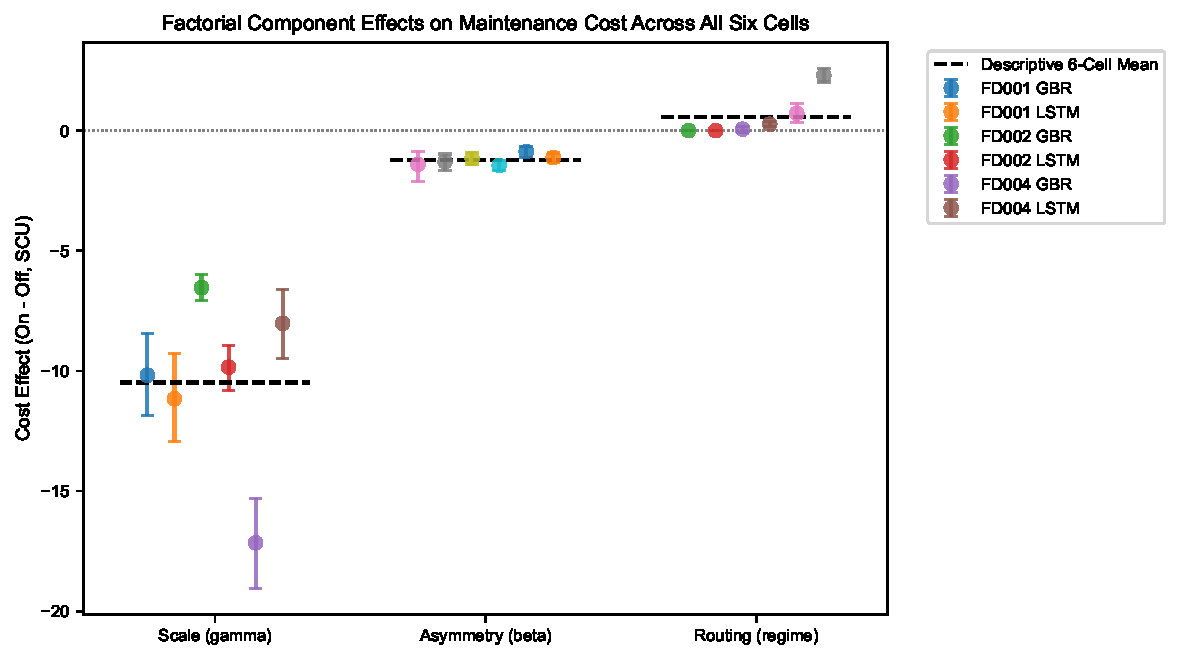
\includegraphics[width=\columnwidth]{figures/scale_asymmetry_routing_paired_effects.pdf}
\caption{Paired main factor effects ($On - Off$) for scale dilation ($\gamma$), directional asymmetry ($\beta$), and operating regime routing across the six dataset/model cells with 10,000-draw stratified bootstrap 95\% confidence intervals.}
\label{fig:factor_effects}
\end{figure}

\begin{figure}[t]
\centering
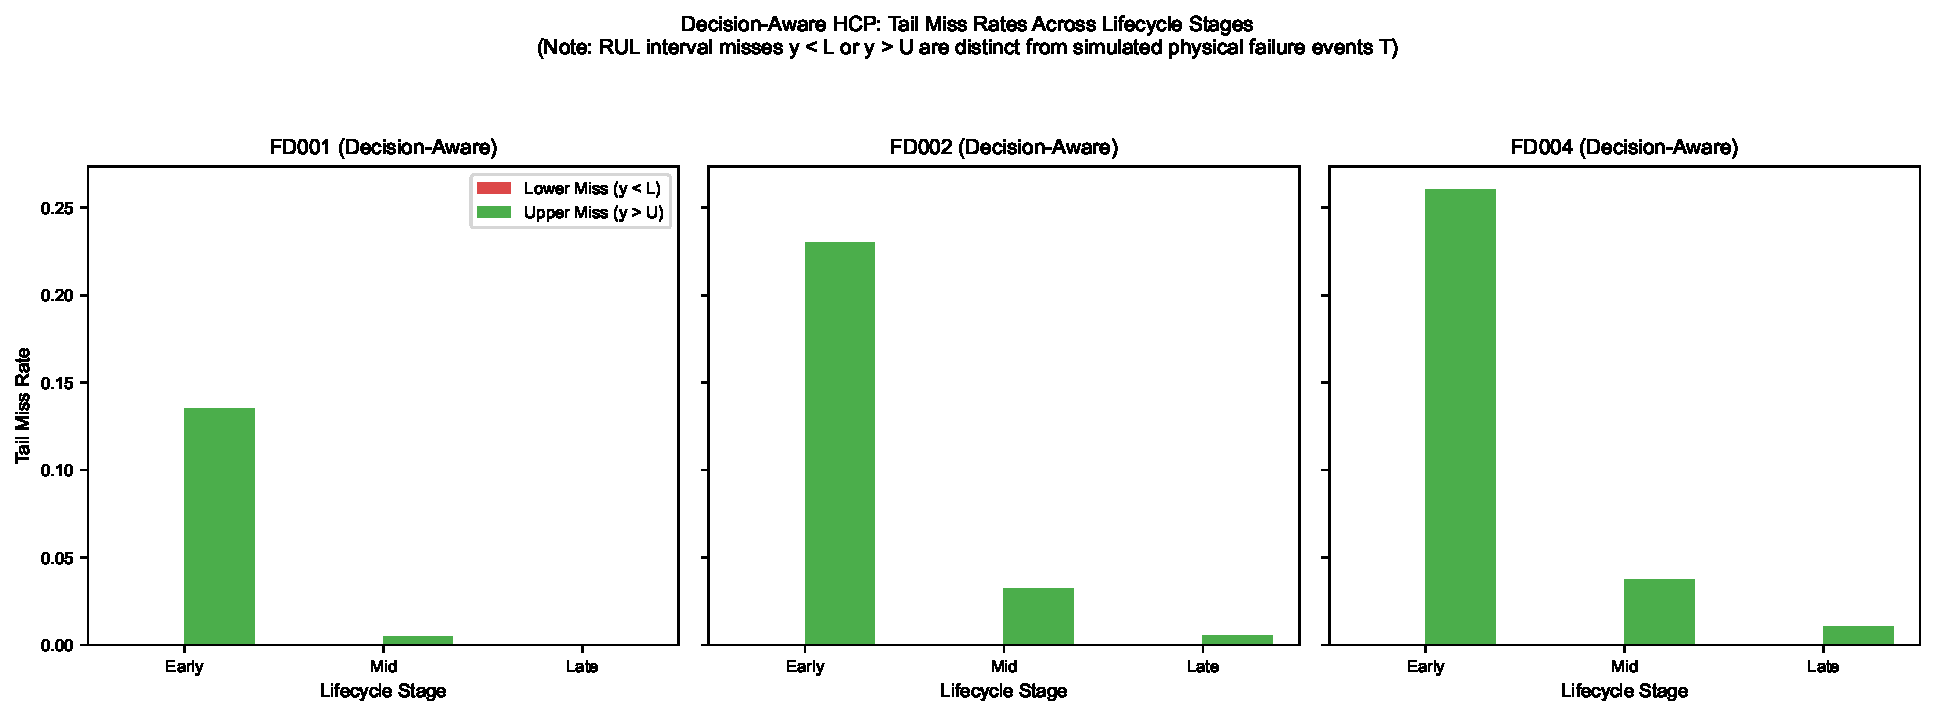
\includegraphics[width=\columnwidth]{figures/lower_upper_miss_rates_by_lifecycle_stage.pdf}
\caption{Empirical lower ($y < L$) vs.\ upper ($y > U$) tail miss rates across early, mid, and late lifecycle stages, illustrating the source of late-life conditional undercoverage.}
\label{fig:miss_rates}
\end{figure}

\subsection{Factorial Main Effects on Maintenance Cost}
As illustrated in Fig.~\ref{fig:factor_effects}:
\begin{itemize}
    \item \textbf{Scale Dilation ($\gamma=2$ vs $0$)}: Yields an unweighted descriptive mean cost reduction of \textbf{-10.4823 SCU} across all 6 cells (range: $-17.16$ to $-6.54$ SCU).
    \item \textbf{Directional Asymmetry ($\beta=-\ln 2$ vs $0$)}: Provides a consistent secondary cost reduction of \textbf{-1.2142 SCU} (range: $-1.44$ to $-0.87$ SCU).
    \item \textbf{Regime Routing (regime vs global)}: Shows an unweighted descriptive mean cost increase of \textbf{+0.5594 SCU}. On FD001, routing has exactly zero effect ($0.0000$ SCU) by mathematical equivalence; on multi-regime datasets, regime partitioning reduces calibration sample density, slightly degrading empirical threshold precision.
\end{itemize}

\subsection{Lifecycle Stage Miss-Rate Asymmetry}
Fig.~\ref{fig:miss_rates} decomposes prediction interval tail misses across early, mid, and late lifecycle stages. In early life ($t \in [w, T/3]$), coverage exceeds 95\% with near-zero lower-tail misses. In late life ($t \in [2T/3, T]$), rapid physical wear acceleration causes increased lower-tail misses ($y < L$), directly explaining the breach of the preregistered $E < 0.05$ worst-stage coverage ceiling.

\subsection{Engineering Stress Robustness Probes}
Under Gaussian sensor noise probes ($\sigma \in \{0.05, 0.10, 0.20\}$ across 54 combinations), mean paired cost increase relative to clean telemetry was $+0.5633$ SCU. Under causal forward-fill sensor dropout ($p \in \{0.05, 0.10\}$ across 36 combinations), mean paired coverage delta was $-0.0007$.

\section{Digital Twin Implementation}

IntelliTwin includes a browser-based historical telemetry replay prototype (`apps/twin_dashboard/`). The prototype operates causally on C-MAPSS validation runs, streaming multi-sensor telemetry, GBR/LSTM point predictions, conformal uncertainty envelopes, and policy decision triggers with zero future lookahead. The implementation was audited and verified to achieve exact numerical parity ($\text{atol} \le 10^{-4}$) against cached validation arrays across all 18 benchmark cells.

\section{Limitations and Threats to Validity}

\subsection{Trade-offs Between Operational Utility and Coverage}
The central insight of this investigation is the fundamental tension between operational maintenance utility and conditional coverage guarantees. By dilating intervals in early life ($\gamma=2$) and skewing bounds downward near end-of-life ($\beta < 0$), IntelliTwin drastically reduced simulated maintenance costs ($+7.50$ to $+11.32$ SCU/engine) and prevented all functional failures. However, this asymmetric tuning sacrificed late-stage conditional coverage ($\sim 77\%$ vs.\ 90\% nominal). In safety-critical engineering, whether this trade-off is acceptable depends entirely on operational risk tolerance.

\subsection{Threats to Validity}
\begin{enumerate}
    \item \textbf{Synthetic Degradation Dynamics}: C-MAPSS is an industry-standard simulation, but real aero-engines experience complex thermomechanical degradation not fully captured in synthetic runs.
    \item \textbf{Synthetic Maintenance Cost Ratios}: The evaluated 1 : 5 : 0.20 cost structure represents an engineering benchmark rather than an airline accounting ledger.
    \item \textbf{Post-Confirmatory Nature of Phase 8}: Phase 8 factorial ablations were designed after inspecting held-out test data. P-values and confidence intervals are reported without multiple-comparison correction.
    \item \textbf{Software Replay Boundary}: The Digital Twin is strictly a validation telemetry replay prototype without physical bi-directional control.
\end{enumerate}

\section{Conclusion and Future Work}

This paper presented IntelliTwin, a decision-aware, condition-adaptive conformal prediction framework for industrial turbofan predictive maintenance. By integrating deep prognostics with state-dependent nonconformity scaling and hierarchical engine weighting, the framework achieved substantial maintenance cost reductions with zero fleet failures. Under a frozen confirmatory protocol, the primary research questions were formally classified as UNSUPPORTED due to conditional coverage degradation in late-life wear stages. Post-confirmatory factorial ablation demonstrated that scale dilation and directional asymmetry drive the observed cost reductions, while operating regime routing introduces variance penalties on multi-condition fleets. Future research will explore online adaptive conformal prediction to restore conditional late-life coverage and investigate fleet-wide collaborative maintenance synchronization.

\section*{Acknowledgment}
The authors express their sincere gratitude to the Department of Information Technology, Ajay Kumar Garg Engineering College (AKGEC), Ghaziabad, and project supervisor Dr. Ruchi Gupta for academic guidance and departmental resources.

\begin{thebibliography}{30}
\providecommand{\url}[1]{#1}
\csname url@samestyle\endcsname
\providecommand{\newblock}{\relax}
\providecommand{\bibinfo}[2]{#2}

\bibitem{benabdennour2026grouped}
A.~BenAbdennour, ``Leakage-controlled grouped validation and interval-safety calibration for RUL/SOH prediction,'' \emph{Machines}, vol.~14, no.~10, p. 1124, 2026.
\bibitem{robinson2026riskaware}
C.~D. Robinson, ``Remaining useful life estimation for aircraft engines with risk-aware prediction intervals,'' \emph{Int. J. Progn. Health Manag.}, vol.~17, no.~1, p. 4724, 2026.
\bibitem{walia2026uncertainty}
G.~K. Walia and M.~Kumar, ``Uncertainty-aware remaining useful life prediction and PPO based optimal maintenance scheduling,'' \emph{Reliab. Eng. Syst. Saf.}, p. 112356, 2026.
\bibitem{yan2026audit}
H.~Yan, ``Conformal prediction intervals for turbofan remaining useful life: an audit across operating regimes,'' \emph{Zenodo}, 2026, doi: 10.5281/zenodo.21330745.
\bibitem{wu2026research}
J.~Wu \emph{et~al.}, ``Research on remaining useful life prediction of equipment based on digital twins,'' \emph{Sensors}, vol.~26, no.~4, p. 1240, 2026.
\bibitem{belay2026digital}
M.~A. Belay, A.~Rasheed, and P.~S. Rossi, ``Digital twin-driven communication-efficient federated anomaly detection for industrial IoT,'' \emph{Preprint, NTNU / IEEE}, 2026.
\bibitem{hisamuddin2026ai}
M.~Hisamuddin, M.~T. Hussain, and R.~Fatima, ``AI-driven digital twins for smart urban infrastructure,'' \emph{Tech. Report, Khaja Bandanawaz Univ.}, 2026.
\bibitem{diao2026turbofan}
R.~Diao, M.~Zhou, G.~Meng, and S.~Wang, ``Turbofan engine remaining useful life prediction with reliable prediction intervals,'' \emph{Sensors}, vol.~26, no.~7, p. 2249, 2026.
\bibitem{yang2026empirical}
S.~Yang, J.~Wang, and Y.~Wang, ``Empirical calibration and conditional-reliability diagnostics for bearing RUL prediction,'' \emph{arXiv:2607.08273}, 2026.
\bibitem{xu2026novel}
W.~Xu, S.~Gao, Z.~Wang, and E.~Zio, ``A novel uncertainty-aware framework for remaining useful life prediction,'' \emph{Reliab. Eng. Syst. Saf.}, vol. 275, p. 112763, 2026.
\bibitem{mahmud2025ai}
A.~K. M.~R. Mahmud \emph{et~al.}, ``AI-augmented digital twin architecture for predictive maintenance,'' \emph{Eur. J. Appl. Sci. Eng. Technol.}, vol.~3, no.~5, pp. 45--58, 2025.
\bibitem{pathri2025smart}
B.~P. Pathri and K.~V. Ganduri, ``From smart cities to manufacturing: A comprehensive study on digital twin applications,'' \emph{IET Digit. Twins Appl.}, vol.~2, p. e70014, 2025.
\bibitem{diana2025ai}
D.~Diana, Putri, and A.~A. Mukti, ``AI-driven digital twin for predictive maintenance in urban infrastructure,'' \emph{Civil Eng. Sci. Technol.}, vol.~1, no.~1, pp. 63--74, 2025.
\bibitem{cortesgomez2025utility}
S.~Cortes-Gomez \emph{et~al.}, ``Utility-directed conformal prediction: A decision-aware framework,'' in \emph{Proc. ICLR}, 2025.
\bibitem{hasan2025new}
S.~K.~K. Hasan and C.~W. Crawford, ``A new era for digital twins: progress and industry adoption,'' \emph{Digital Twin}, vol.~2, no.~4, p. 2555877, 2025.
\bibitem{zhu2025predictive}
Z.~Zhu \emph{et~al.}, ``Predictive maintenance strategies for aero-engines considering remaining useful life prediction interval,'' \emph{Qual. Reliab. Eng. Int.}, 2025.
\bibitem{brighenti2024forecasting}
F.~Brighenti \emph{et~al.}, ``Forecasting bridge damage within a predictive Structural Reliability-based DSS,'' \emph{Autom. Constr.}, vol. 168, p. 105740, 2024.
\bibitem{shehadeh2024evaluating}
H.~K. Shehadeh, ``Evaluating the impact of transitioning maintenance strategy from reactive to proactive,'' \emph{WSEAS Trans. Bus. Econ.}, vol.~21, pp. 838--856, 2024.
\bibitem{wei2024digital}
H.~Wei, ``Digital twin and AI enabled predictive maintenance in building industry,'' Ph.D. dissertation, Nanyang Technological University, Singapore, 2024.
\bibitem{bello2024ai}
S.~F. Bello \emph{et~al.}, ``AI-driven predictive maintenance and optimization of renewable energy systems,'' \emph{Int. J. Sci. Res. Arch.}, vol.~13, no.~1, pp. 2823--2837, 2024.
\bibitem{mazzetto2024review}
S.~Mazzetto, ``A review of urban digital twins integration, challenges, and future directions,'' \emph{Sustainability}, vol.~16, no.~19, p. 8337, 2024.
\bibitem{mousavi2024evolution}
V.~Mousavi \emph{et~al.}, ``Evolution of digital twin frameworks in bridge management,'' \emph{Remote Sens.}, vol.~16, no.~11, p. 1887, 2024.
\bibitem{hosseinzadeh2023predictive}
A.~Hosseinzadeh \emph{et~al.}, ``A predictive maintenance approach in manufacturing systems via AI-based early failure detection,'' \emph{Mfg. Lett.}, vol.~35, pp. 1179--1186, 2023.
\bibitem{javanmardi2023conformal}
A.~Javanmardi and E.~H{\"u}llermeier, ``Conformal prediction intervals for remaining useful lifetime estimation,'' \emph{Int. J. Progn. Health Manag.}, vol.~14, no.~2, p. 3417, 2023.
\bibitem{lee2023hierarchical}
Y.~Lee, R.~F. Barber, and R.~Willett, ``Distribution-free inference with hierarchical data,'' \emph{arXiv:2306.06342v4}, 2023.
\bibitem{chen2022data}
C.~Chen \emph{et~al.}, ``Data-driven predictive maintenance strategy considering the uncertainty in remaining useful life prediction,'' \emph{Neurocomputing}, vol. 494, pp. 79--88, 2022.
\bibitem{huang2021survey}
Z.~Huang, Y.~Shen, J.~Li, M.~Fey, and C.~Brecher, ``A survey on AI-driven digital twins in Industry 4.0,'' \emph{Sensors}, vol.~21, no.~19, p. 6340, 2021.
\bibitem{lakens2017equivalence}
D.~Lakens, ``Equivalence tests: A practical primer for t tests, correlations, and meta-analyses,'' \emph{Soc. Psychol. Personal. Sci.}, vol.~8, no.~4, pp. 355--362, 2017.
\bibitem{saxena2008damage}
A.~Saxena, K.~Goebel, D.~Simon, and N.~Eklund, ``Damage propagation modeling for aircraft engine run-to-failure simulation,'' in \emph{Proc. IEEE PHM}, 2008, pp. 1--9.
\bibitem{gneiting2007strictly}
T.~Gneiting and A.~E. Raftery, ``Strictly proper scoring rules, prediction, and estimation,'' \emph{J. Am. Stat. Assoc.}, vol. 102, no. 477, pp. 359--378, 2007.

\end{thebibliography}

\end{document}

